\documentclass[../manuscript.tex]{subfiles}
\section{Полученные результаты}
При разработке данного метода его валидация проводилась на задаче химического перепрограммирования. Валидация метода была выполнена на 6 клеточных переходах из базы данных CFM. Ниже приведена таблица \ref{cell_conv} с указанием для них исходной и конечной клеточной линии, а также количества протоколов в базе CFM. 
\begin{table}[h]
    \caption{Рассмотренные клеточные переходы базы данных CFM}
    \centering
    \begin{tabular}{|c|c|c|c|}
    \hline
          \makecell{№ клет. \\перехода} & \makecell{Исходная \\клеточная линия} & \makecell{Конечная\\ клеточная линия} & \makecell{количество\\ протоколов} \\
         \hline
         1 & фибробласты & \makecell{индуцированные \\кардиомиоциты} & 19 \\
         \hline
         2 &фибробласты & \makecell{индуцированные \\нейроны }& 8 \\
         \hline 
         3 & фибробласты & \makecell{индуцированные \\нейральные стволовые клетки} & 6 \\
         \hline 
         4 & фибробласты & \makecell{индуцированные \\ $ \beta$-клетки поджелудочной железы} & 6 \\
         \hline 
         5 & \makecell{мезенхимальные \\стволовые клетки} & \makecell{индуцированные нейроны} & 5 \\
         \hline
         6 & фибробласты & \makecell{индуцированные \\плюрипотентные стволовые клетки} & 4 \\
         \hline 
    \end{tabular}
    \label{cell_conv}
\end{table}
\subsection{Оптимизация метода, основанного на сравнении \\экспрессионных сигнатур, и его валидация}

Одним из важных этапов разработки метода было определение значений коэффициентов в выражении inf\_score.
При помощи байесовской оптимизации были определены коэффициенты в выражении inf\_score для каждого клеточного перехода. Эти коэффициенты соответствовали максимуму разницы средних значений уровня синергии для синергетических пар и несинергетических пар. В качестве оптимальных значений коэффициентов метрик взяли средние значения определенных коэффициентов метрик при байесовской оптимизации по всем клеточным переходам. Ниже в таблице \href{coeff_table} приведены эти значения коэффициентов.


\begin{table}[h]
    \caption{Рассмотренные клеточные переходы базы данных CFM}
    \centering
    \begin{tabular}{|c|c|c|c|c|c|c|c|}
    \hline
\makecell{№ клет. \\перехода}  & \makecell{coeff\\Btw} & \makecell{coeff\\Cln} & \makecell{coeff\\Egt} & \makecell{coeff\\Egv} & \makecell{coeff\\Ktz} & \makecell{coeff\\|logFC|} & \makecell{coeff\\Prk }\\
\hline
1        &                9.8498 &          4.6486 &           9.4933 &            9.5533 &     9.7345 &      1.0621 &         9.4915 \\
\hline
2                 &            4.1706 &          4.2732 &           5.3341 &            3.5209 &     6.2944 &      2.7864 &         9.9804 \\
\hline
3      &              9.8498 &          4.6486 &           9.4933 &            9.5533 &     9.7345 &      1.0621 &         9.4915 \\
\hline
4 &             9.5985 &          9.6596 &           9.2349 &            1.2538 &       9.53 &      1.4785 &         7.2369 \\
\hline
5  &           9.0555 &          8.3232 &           9.1446 &            9.6125 &     9.8218 &       9.867 &         7.4246 \\
\hline


6 &            8.7357 &          1.6625 &           9.9294 &            9.8643 &     9.3573 &      1.2376 &         1.2547 \\
\hline


\makecell{opt.\\ coeff} &    8.5433 &          5.5359 &           8.7716 &            7.2264 &     9.0787 &      2.9156 &         7.4799 \\
\hline
    \end{tabular}
    \label{coeff_table}
\end{table}
В целом наблюдается некоторое постоянство коэффициентов для метрик. Например, для метрик betweenness(Btw), eigentrust (Egt),  Katz centrality (Ktz), |logFC| наблюдается маленький разброс коэффициентов.  По полученным коэффициентам можно сказать, что большой вес имеют метрики betweenness(Btw), eigentrust (Egt), eigenvector centrality (Egv), Katz centrality (Ktz), pagerank (Prk). Метрика |logFC| обладает наименьшим весом. 

Также в таблице \ref{coeff_max} для этих валидаций приведены величины, которые показывают успешность метода : разница средних значений уровня синергии для синергетических пар и несинергетических пар, p-значение, определяемое тестом Колмогорова-Смирнова. Разница средних значений уровня синергии для синергетических пар и несинергетических пар рассчиталась как:
\begin{equation}
    d = \bar{synergy\_score_{syn}} - \bar{synergy\_score_{not\_syn}}
    \label{equation1}
\end{equation}
Ожидается, что разница средних значений уровня синергии для синергетических пар и несинергетических пар для всех клеточных переходов будет положительна, поскольку, чем выше уровень синергии, тем выше синергетический эффект. 


Поскольку список пар ранжируется по вычисленному уровню синергии, то следующие метрики: число синергетических пар среди первых 50 пар, число синергетических пар среди первых пар, составляющих 5\% от всех пар, доля синергетических пар среди первых пар, составляющих 5\% от всех пар, - были показательны. 



\begin{table}[h]
    \caption{Результаты валидации на коэффициентах, определенных при байесовской оптимизации}
    \centering
    \begin{tabular}{|c|c|c|c|c|c|c|c|}
    \hline
    \makecell{№ кл. \\перех.}  &  \makecell{разн. \\ср. знач.} &       p\_value &   \makecell{число \\синерг.\\ пар\\ в топ 50} &   \makecell{число \\пар }&   \makecell{число \\синерг. \\пар \\в топ 5\% }&  \makecell{ число\\ пар \\в топ 5\%} &  \makecell{ доля \\синерг.\\ пар\\ в топ 5\% }\\
\hline
1 &           0.0218 &  0 &                          15 &    1236378 &                   33287 &           61819 &               0.538\\
\hline
2 &           0.0086 &  8.095e-12 &                          37 &      71631 &                    2581 &            3582 &               0.721 \\
\hline
3 &           0.0469 &  0 &                          26 &     475800 &                   17560 &           23790 &               0.738 \\
\hline
4 &           0.0084 &  4.409e-10 &                          22 &      74691 &                    1552 &            3735 &               0.416 \\
\hline
5 &           0.0124 &  3.455e-42 &                          40 &      49770 &                    1525 &            2488 &               0.613 \\
\hline
6 &          -0.0199 &  1.990e-60 &                          37 &     128778 &                    3590 &            6439 &               0.558\\
\hline
    \end{tabular}
    \label{coeff_max}
\end{table}
Стоит сразу отметить, что p-значение, определяемое тестом Колмогорова-Смирнова, достаточное низкое, что позволяет отвергнуть гипотезу, что выборки значений уровня синергии для синергетических и несинергетических пар принадлежат одному распределению. Таким образом метод разделяет синергетические и несинергетические пары. Для 5 клеточных переходов разница средних значений уровней синергии синергетических пар и несинергетических пар положительна. Она отрицательна только для перехода из фибробластов в индуцированные плюрипотентные стволовые клетки.


На рисунке \ref{cos_dist_max} показаны распределения значений уровня синергии для синергетических пар и несинергетических пар.

\begin{figure}[H]
\begin{minipage}[h]{0.5\linewidth}
\center{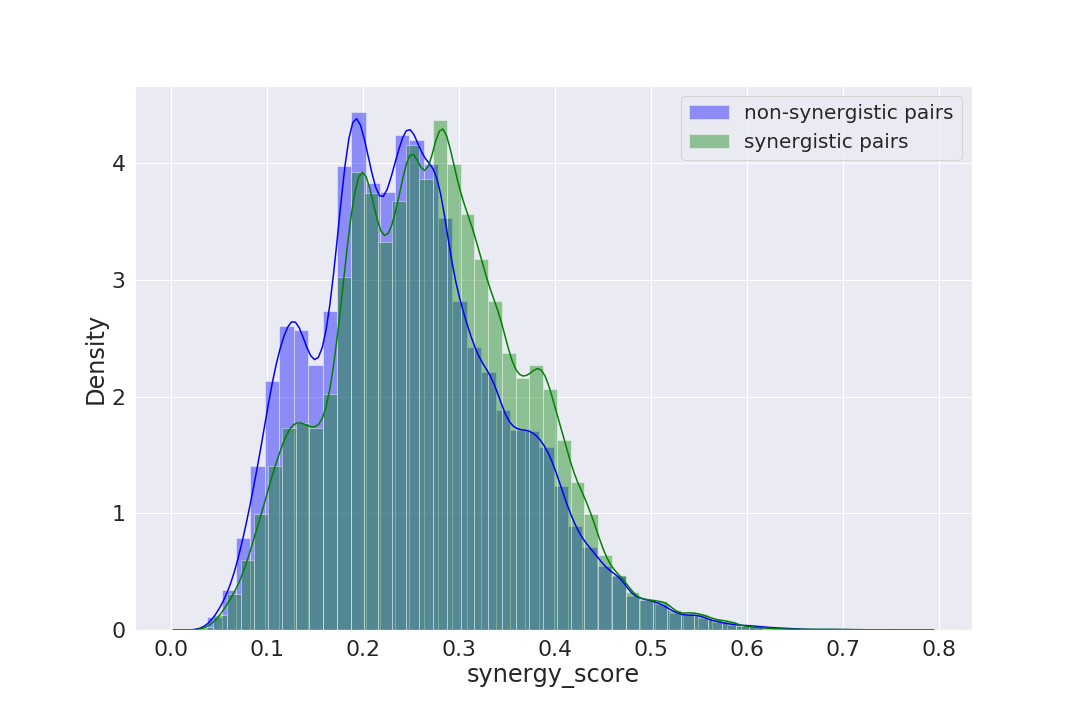
\includegraphics[width=1\linewidth]{images/fig_cosine_dist_Fibroblasts_Induced_Cardiomyocytes_max_big_label.png}} a) \\
\end{minipage}
\hfill
\begin{minipage}[h]{0.5\linewidth}
\center{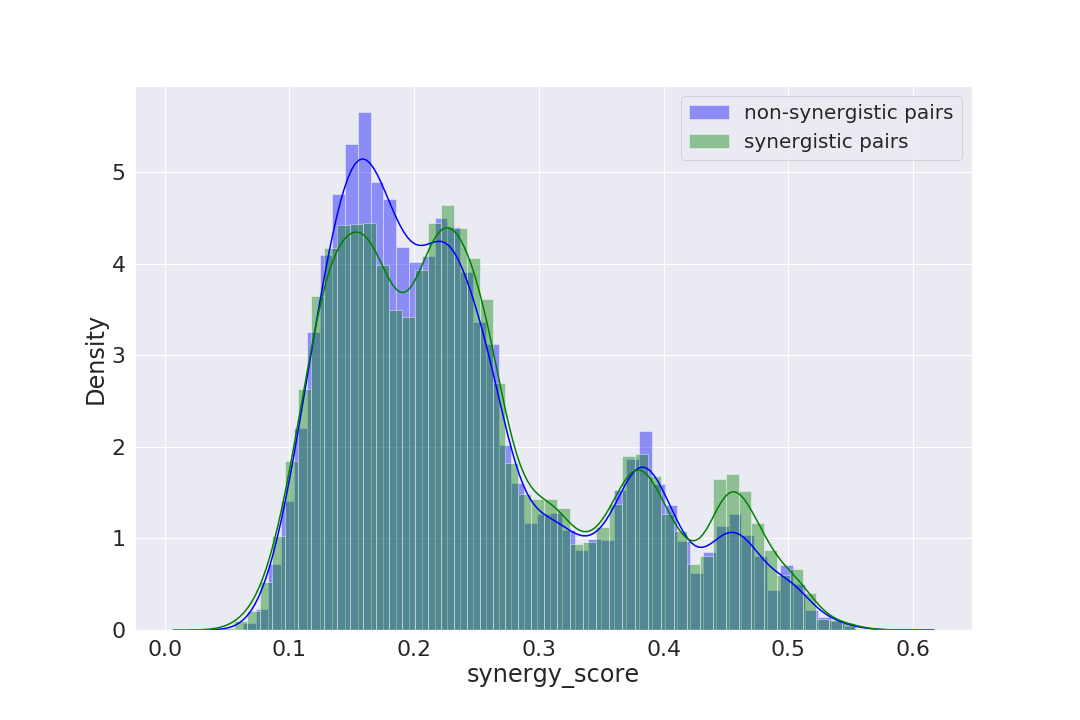
\includegraphics[width=1\linewidth]{images/fig_cosine_dist_Fibroblasts_Induced_Neurons_max_big_label.png}} \\b)
\end{minipage}
\vfill
\begin{minipage}[h]{0.5\linewidth}
\center{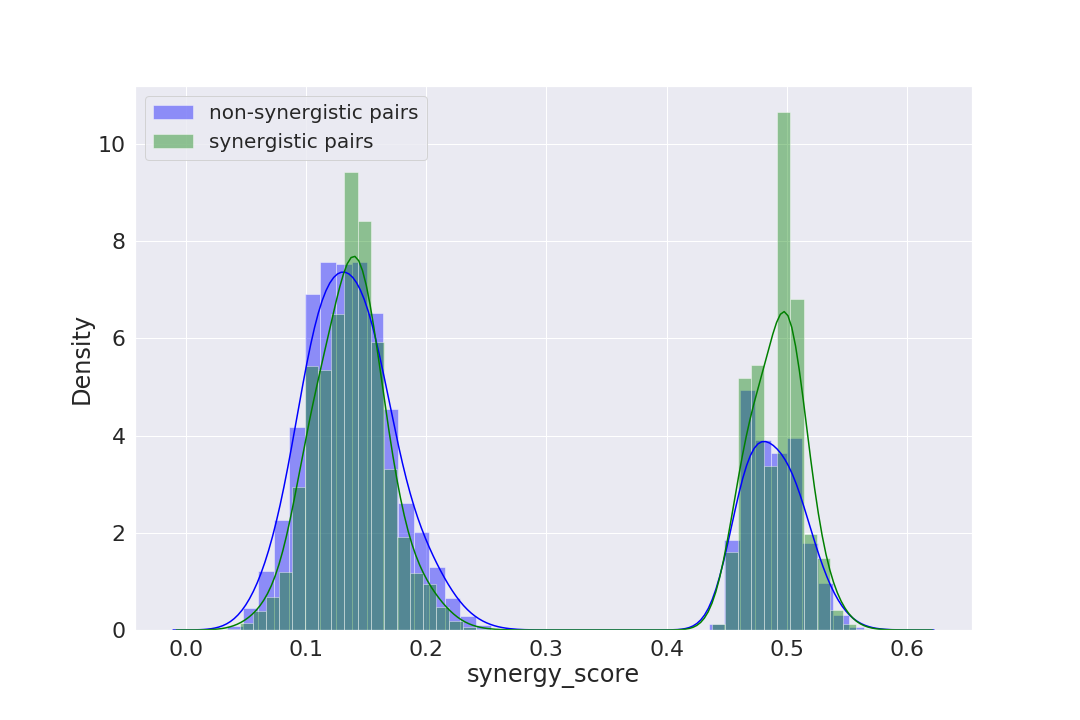
\includegraphics[width=1\linewidth]{images/fig_cosine_dist_Fibroblasts_Induced_Neural_Stem_Cells_max_big_label.png}} c) \\
\end{minipage}
\hfill
\begin{minipage}[h]{0.5\linewidth}
\center{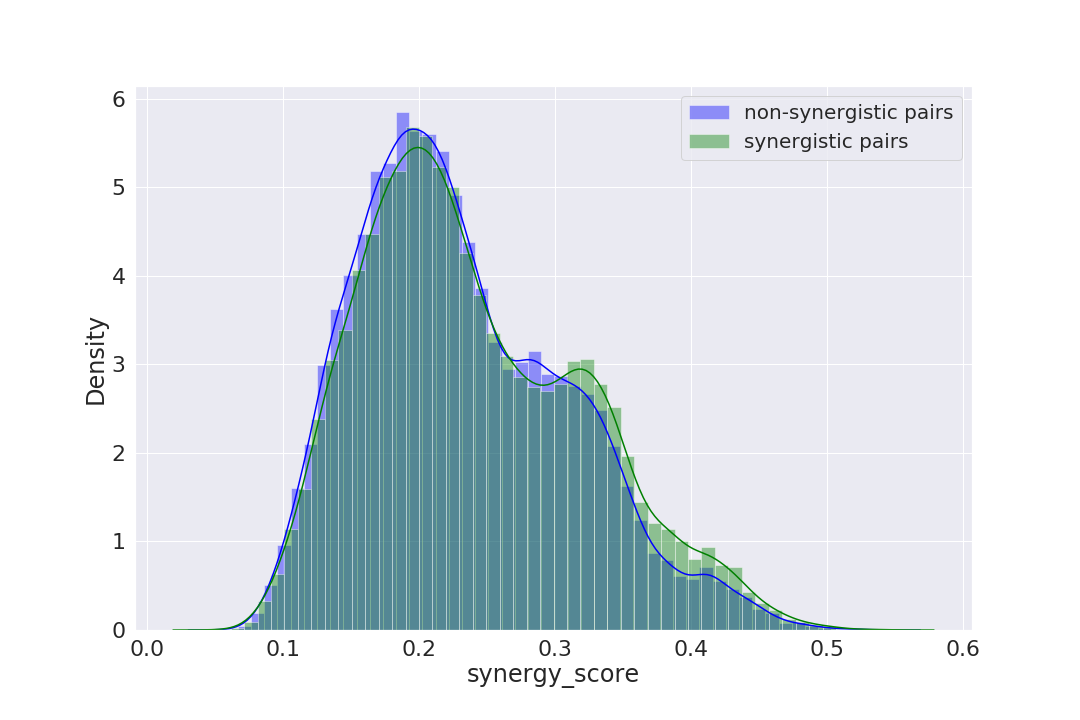
\includegraphics[width=1\linewidth]{images/fig_cosine_dist_Fibroblasts_Induced_Pancreatic_Beta_Cells_max_big_label.png}} d) \\
\end{minipage}
\vfill
\begin{minipage}[h]{0.5\linewidth}
\center{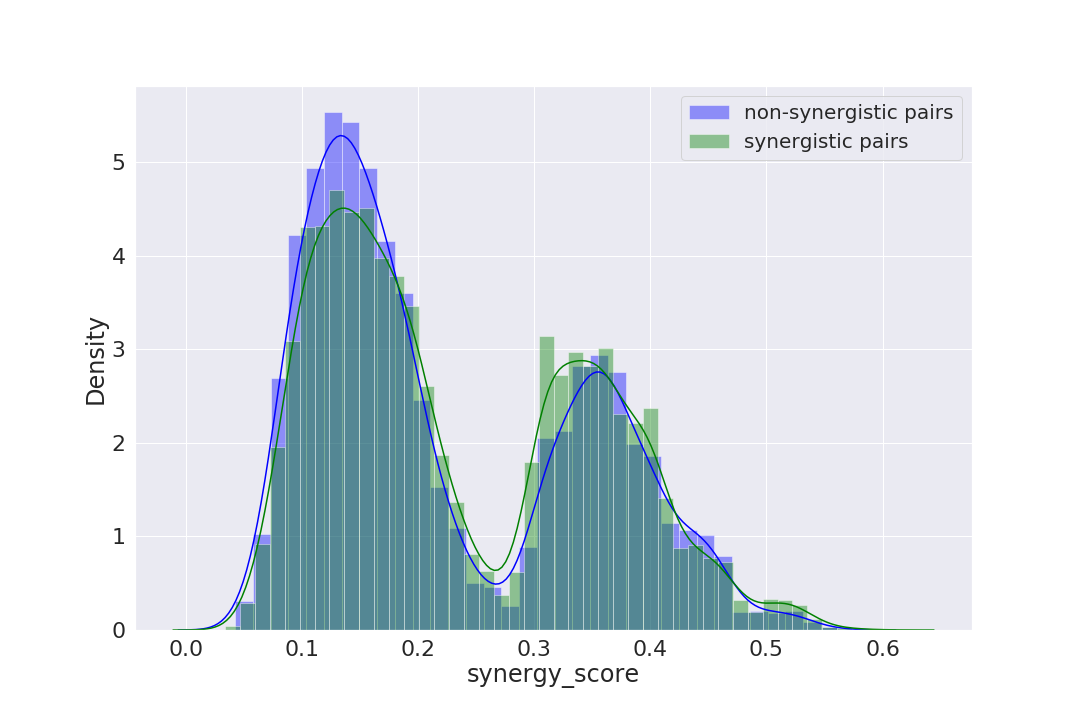
\includegraphics[width=1\linewidth]{images/fig_cosine_dist_Mesenchymal_Stem_Cells_Induced_Neurons_max_big_label.png}} e) \\
\end{minipage}
\hfill
\begin{minipage}[h]{0.5\linewidth}
\center{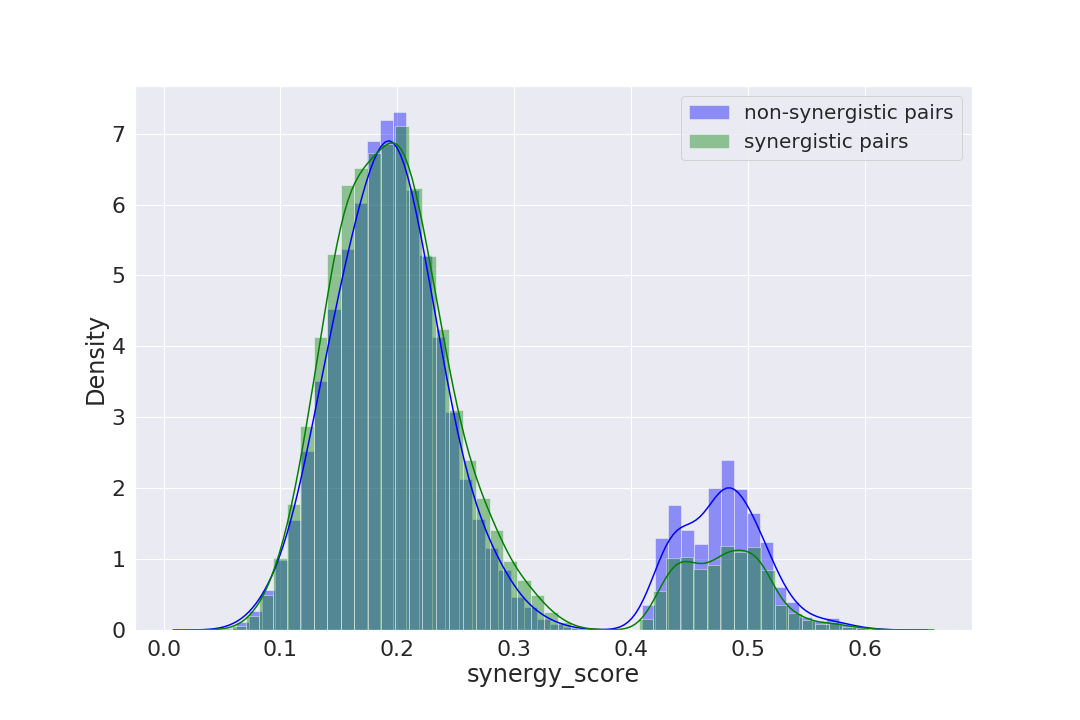
\includegraphics[width=1\linewidth]{images/fig_cosine_dist_Fibroblasts_Induced_Pluripotent_Stem_Cells_max_big_label.png}} f)
\end{minipage}
\caption{Распределение значений уровня синергии синергетических и несинергетических пар : a) фибробласты -> индуцированные кардиомиоциты, b)фибробласты -> индуцированные нейроны c) фибробласты -> индуцированные нейральные стволовые клетки, d)  фибробласты -> индуцированные $ \beta$-клетки поджелудочной железы, e) мезенхимальные стволовые клетки -> индуцированные нейроны, f) фибробласты -> индуцированные плюрипотентные стволовые клетки }
\label{cos_dist_max}
\end{figure}

Чтобы проверить оптимальные коэффициенты в выражении inf\_score, была проведена валидация с этим набором коэффициентов на 6 клеточных переходах. В таблице приведены результаты валидации. 

\begin{table}[h]
    \caption{Результаты валидации на оптимальных коэффициентах}
    \centering
    \begin{tabular}{|c|c|c|c|c|c|c|c|}
    \hline
    \makecell{№ кл. \\перех.}  &  \makecell{разн. \\ср. знач.} &       p\_value &   \makecell{число \\синерг.\\ пар\\ в топ 50} &   \makecell{число \\пар }&   \makecell{число \\синерг.\\ пар \\в топ 5\% }&  \makecell{ число\\ пар \\в топ 5\%} &  \makecell{ доля \\синерг.\\ пар\\ в топ 5\% }\\
\hline
1 &           0.0203 &  0 &                          11 &    1236378 &                   33108 &           61819 &               0.536 \\
\hline
2 &           0.0115 &  4.667e-10 &                          37 &      71631 &                    2566 &            3582 &               0.716 \\
\hline
3 &           0.0422 &  0 &                          23 &     475800 &                   16889 &           23790 &               0.710 \\
\hline
4 &           0.0068 &  8.492e-08 &                          18 &      74691 &                    1471 &            3735 &               0.394 \\
\hline
5 &           0.0068 &  4.840e-38 &                          42 &      49770 &                    1558 &            2488 &               0.626 \\
\hline
6 &          -0.0221 &  1.595e-60 &                          34 &     128778 &                    3559 &            6439 &               0.553 \\
\hline
    \end{tabular}
    \label{coeff_table}
\end{table}

При валидации на оптимальных коэффициентах для всех переходов p-значения также достаточно низкие. Характер смещения выборки значений уровня синергии для синергетических пар относительно выборки значений уровня синергии несинергетических пар остался прежним. 


На рисунке \ref{cos_dist_opt} показаны распределения значений уровня синергии для синергетических пар и несинергетических пар.

\begin{figure}[H]
\begin{minipage}[h]{0.5\linewidth}
\center{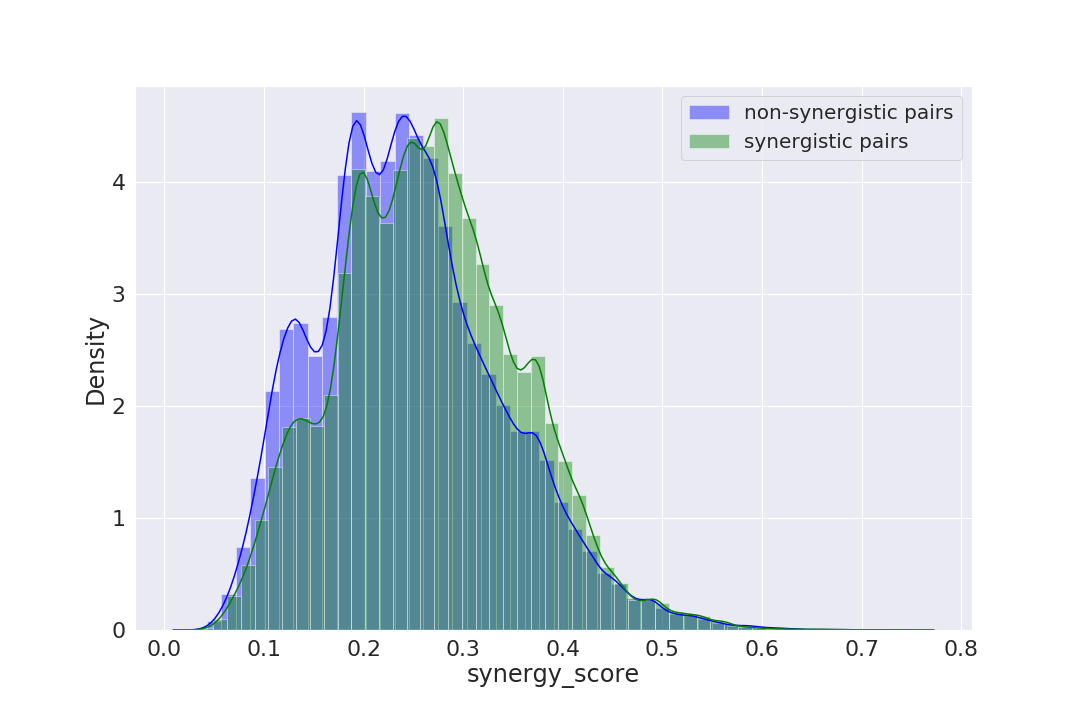
\includegraphics[width=1\linewidth]{images/fig_cosine_dist_Fibroblasts_Induced_Cardiomyocytes_opt_big_label.png}} a) \\
\end{minipage}
\hfill
\begin{minipage}[h]{0.5\linewidth}
\center{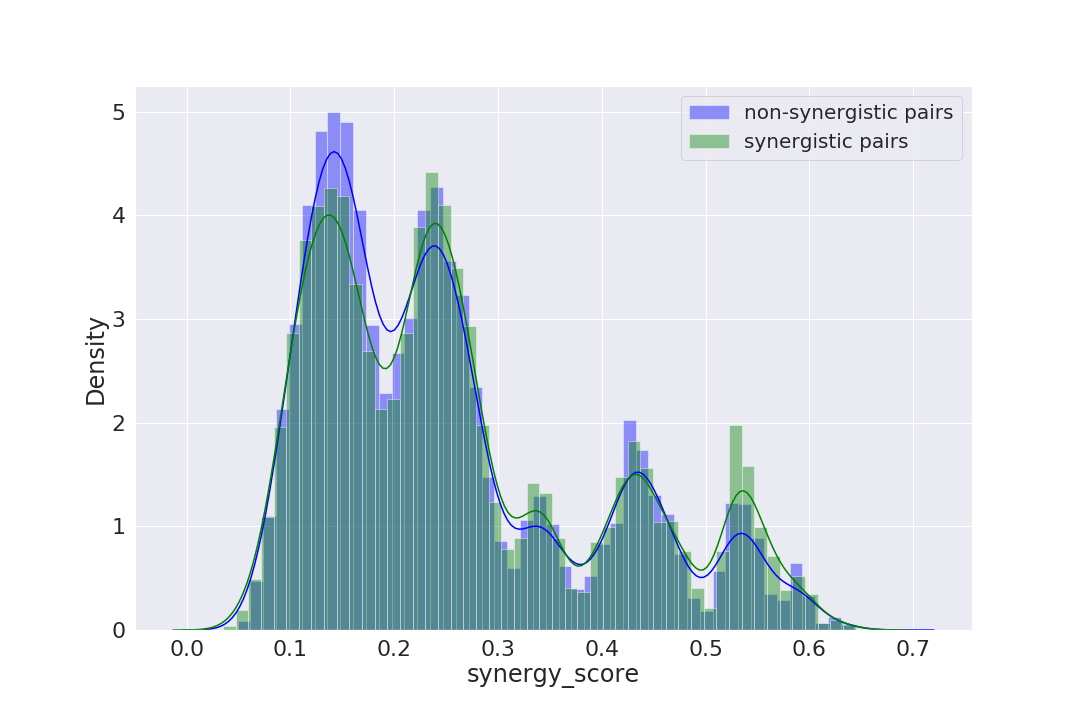
\includegraphics[width=1\linewidth]{images/fig_cosine_dist_Fibroblasts_Induced_Neurons_opt_big_label.png}} \\b)
\end{minipage}
\vfill
\begin{minipage}[h]{0.5\linewidth}
\center{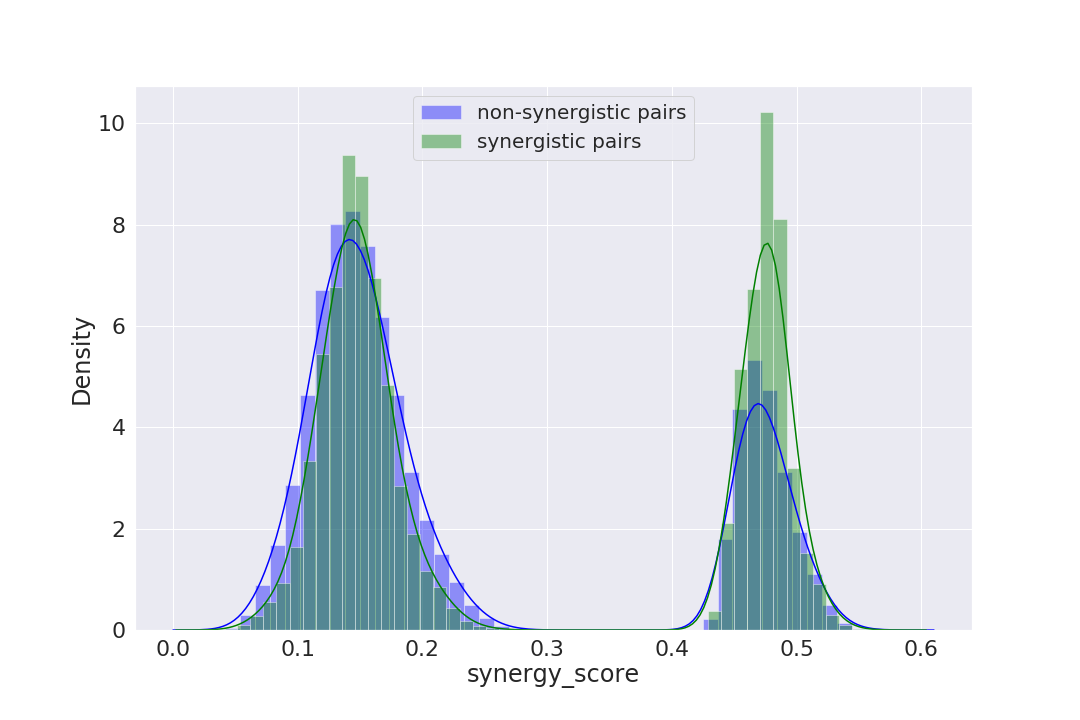
\includegraphics[width=1\linewidth]{images/fig_cosine_dist_Fibroblasts_Induced_Neural_Stem_Cells_opt_big_label.png}} c) \\
\end{minipage}
\hfill
\begin{minipage}[h]{0.5\linewidth}
\center{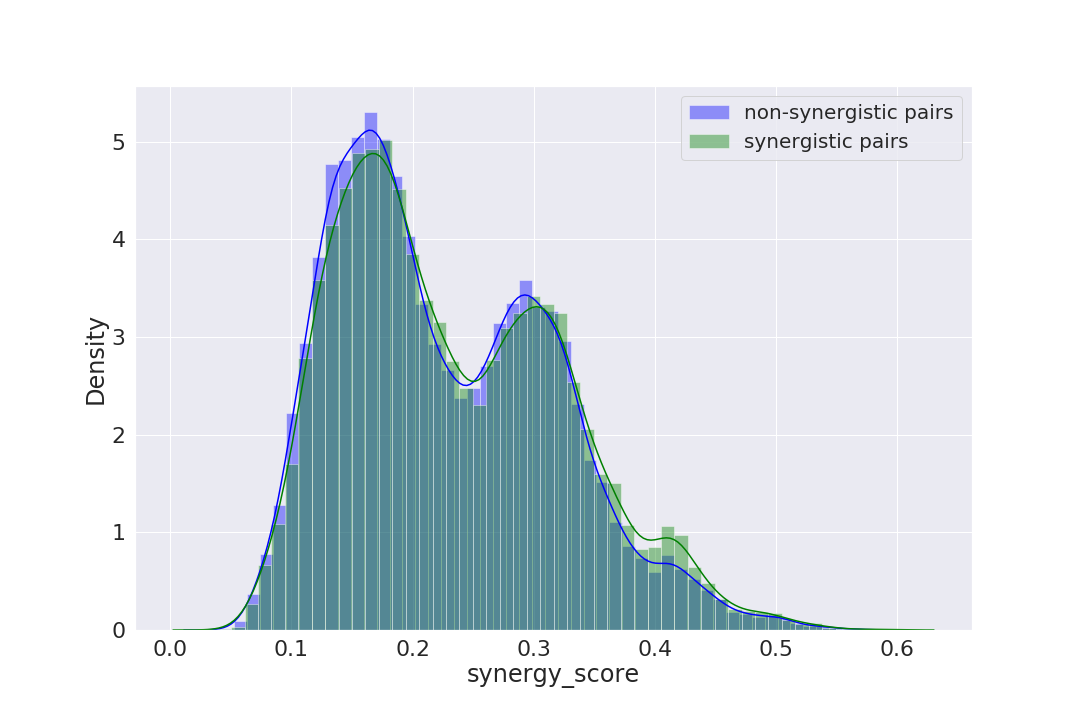
\includegraphics[width=1\linewidth]{images/fig_cosine_dist_Fibroblasts_Induced_Pancreatic_Beta_Cells_opt_big_label.png}} d) \\
\end{minipage}
\vfill
\begin{minipage}[h]{0.5\linewidth}
\center{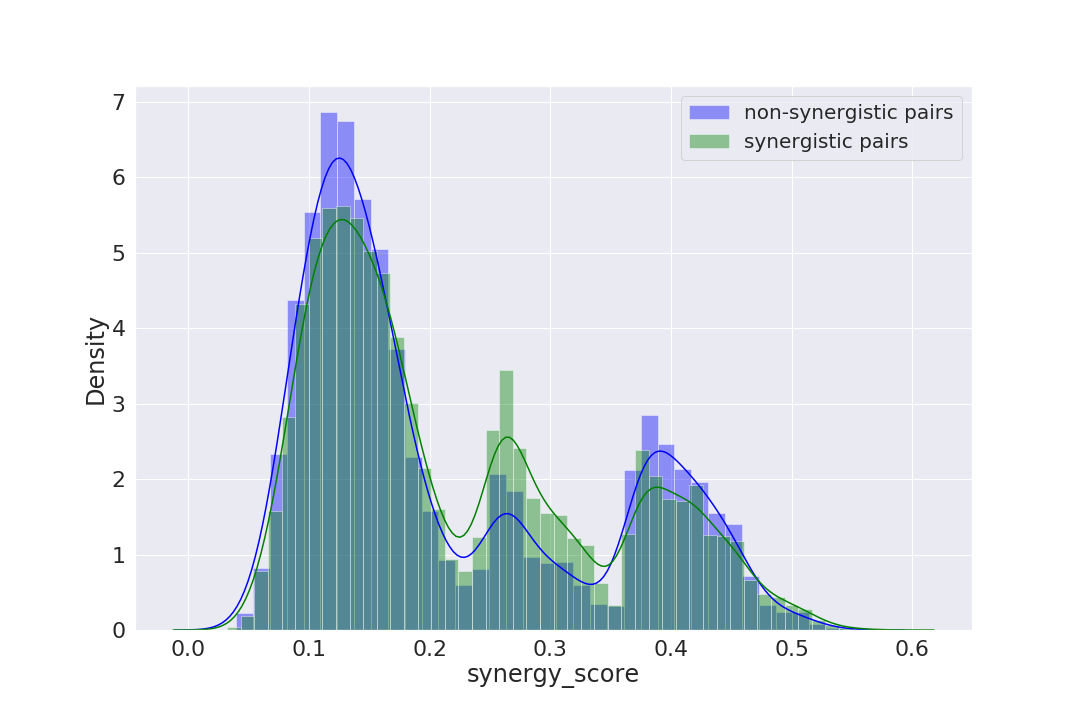
\includegraphics[width=1\linewidth]{images/fig_cosine_dist_Mesenchymal_Stem_Cells_Induced_Neurons_opt_big_label.png} e) \\
\end{minipage}
\hfill
\begin{minipage}[h]{0.5\linewidth}
\center{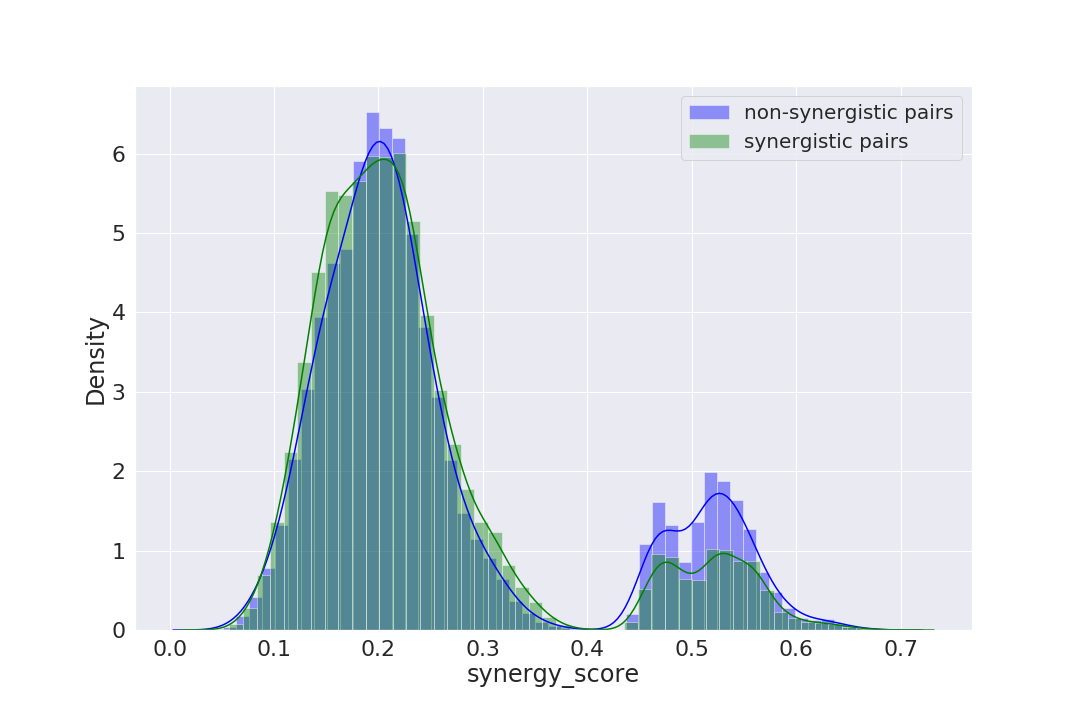
\includegraphics[width=1\linewidth]{images/fig_cosine_dist_Fibroblasts_Induced_Pluripotent_Stem_Cells_opt_big_label.png}} f)
\end{minipage}
\caption{Распределение значений уровня синергии синергетических и несинергетических пар : a) фибробласты -> индуцированные кардиомиоциты, b)фибробласты -> индуцированные нейроны c) фибробласты -> индуцированные нейральные стволовые клетки, d)  фибробласты -> индуцированные $ \beta$-клетки поджелудочной железы, e) мезенхимальные стволовые клетки -> индуцированные нейроны, f) фибробласты -> индуцированные плюрипотентные стволовые клетки }
\label{cos_dist_opt}
\end{figure}

Сравним результаты валидации на оптимальных коэффициентах и коэффициентах, определенных при байесовской оптимизации. В таблице \ref{compare_table} приведены относительные изменения следующих величин : разница средних значений уровня синергии для синергетических пар и несинергетических пар, число синергетических пар в топ 50 пар, число синергетических пар в топ 5\% пар.

\begin{table}[h]
    \caption{Сравнение результатов валидации}
    \centering
    \begin{tabular}{|c|c|c|c|}
\hline
\makecell{№ клет. \\перехода}  &  \makecell{отн. изм. \\разн. \\ср. знач.} &  \makecell{отн. изм.\\ числа \\синерг. пар \\в топ 50 пар} &  \makecell{отн. изм.\\ числа \\синерг. пар\\ в топ 5\% пар }\\
\hline
1 &                -0.069 &                            -0.267 &                      -0.005 \\
\hline
2 &                  0.337&                                    0 &                       -0.006 \\
\hline
3 &                 -0.100 &                            -0.115 &                       -0.038\\
\hline
4 &                 -0.190 &                            -0.182 &                       -0.052 \\
\hline
5 &                 -0.452 &                                 0.05 &                        0.021 \\
\hline
6 &                  0.111 &                           -0.081 &                       -0.009 \\
\hline
    \end{tabular}
    \label{compare_table}
\end{table}
Как и ожидалось, для большинства переходов результаты ухудшились, поскольку наборы коэффициентов, полученные при байесовской оптимизации, были подобраны под каждый переход. Если смотреть на относительное изменение разницы средних значений, то сильнее всего эта величина снизилась для перехода из мезенхимальных стволовых клеток в индуцированные нейроны (на 45\%). Для остальных она упала меньше, чем на 20\%, или повысилась. Для числа синергетических пар в топ 50 пар снижение составляло не более 30 \%.  Снижение числа синергетических пар в топ 5\% пар не превышало 6\%. Эти результаты показывают, что оптимальные коэффициенты подходят всем рассмотренным клеточным переходам.
\subsection{Валидация метода, основанного на сравнении \\ обогащенных сигнальных путей}
Также была проведена валидация с целью проверки эффективности метода при вычислении уровня синергии на основе сравнения обогащенных сигнальных путей. Было проверено 2 способа расчета уровня синергии.
\subsubsection{С использованием коэффициента Танимото}
Данный подход проверяет гипотезу, что синергетические малые молекулы, дополняя друг друга, затрагивают сигнальные пути, полученные в результате анализа обогащения генов с повышенной экспрессией и генов с пониженной экспрессией сигнатуры запроса. То есть, синергетические малые молекулы совместно охватывают все нужные клеточные процессы. 
Была выполнена валидация метода с разными метриками оценки его эффективности. В таблице \ref{tanimoto_table} показаны ее результаты .
\begin{table}[h]
    \caption{Результаты валидации}
    \centering
    \begin{tabular}{|c|c|c|c|c|c|c|c|}
    \hline
    \makecell{№ кл. \\перех.}  &  \makecell{разн.\\ ср. знач.} &        p\_value &  \makecell{число \\ синерг.\\ пар \\ в топ 50 }&  \makecell{число \\пар} &  \makecell{число \\синерг.\\ пар \\в топ 5\%} &  \makecell{число\\ пар \\в топ 5\% } &  \makecell{доля \\синерг.\\ пар \\в топ 5\%}\\
\hline
1 &          -0.0011 &  7.522e-193 &                          23 &    1236378 &                   25300 &           61819 &               0.409 \\
\hline
2 &          -0.0011 &   2.684e-05 &                          22 &      71631 &                    2356 &            3582 &               0.658 \\
\hline
3 &           0.0052 &  6.020e-244 &                          35 &     475800 &                   18451 &           23790 &               0.778 \\
\hline
4 &           0.0018 &   1.096e-10 &                          38 &      74691 &                    1523 &            3735 &               0.408 \\
\hline
5 &           0.0001 &   1.950e-02 &                          31 &      49770 &                    1457 &            2488 &               0.586 \\
\hline
6 &          -0.0022 &   2.949e-26 &                          27 &     128778 &                    3967 &            6439 &               0.616\\
\hline
    \end{tabular}
    \label{tanimoto_table}
\end{table}
P-значения достаточно низкие для всех клеточных переходов, как и в предыдущем методе. Однако разница средних значений синергии синергетических и несинергитических пар отрицательна для 3 клеточных переходов. По этому показателю можно сказать, что данный подход хуже метода, основанного на экспрессионных сигнатурах и генных сетях .



На рисунке \ref{tanimoto} показаны распределения значений уровня синергии для синергетических пар и несинергетических пар.
\begin{figure}[H]
\begin{minipage}[h]{0.5\linewidth}
\center{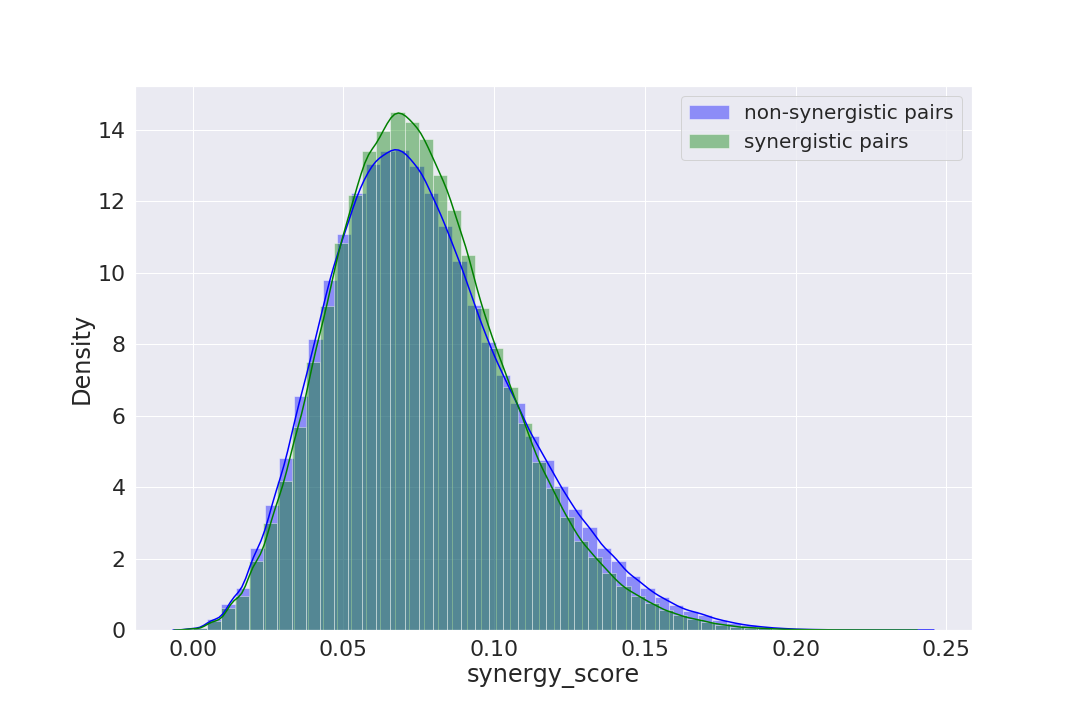
\includegraphics[width=1\linewidth]{images/fig_tanimoto_coeff_Fibroblasts_Induced_Cardiomyocytes_opt_big_label.png}} a) \\
\end{minipage}
\hfill
\begin{minipage}[h]{0.5\linewidth}
\center{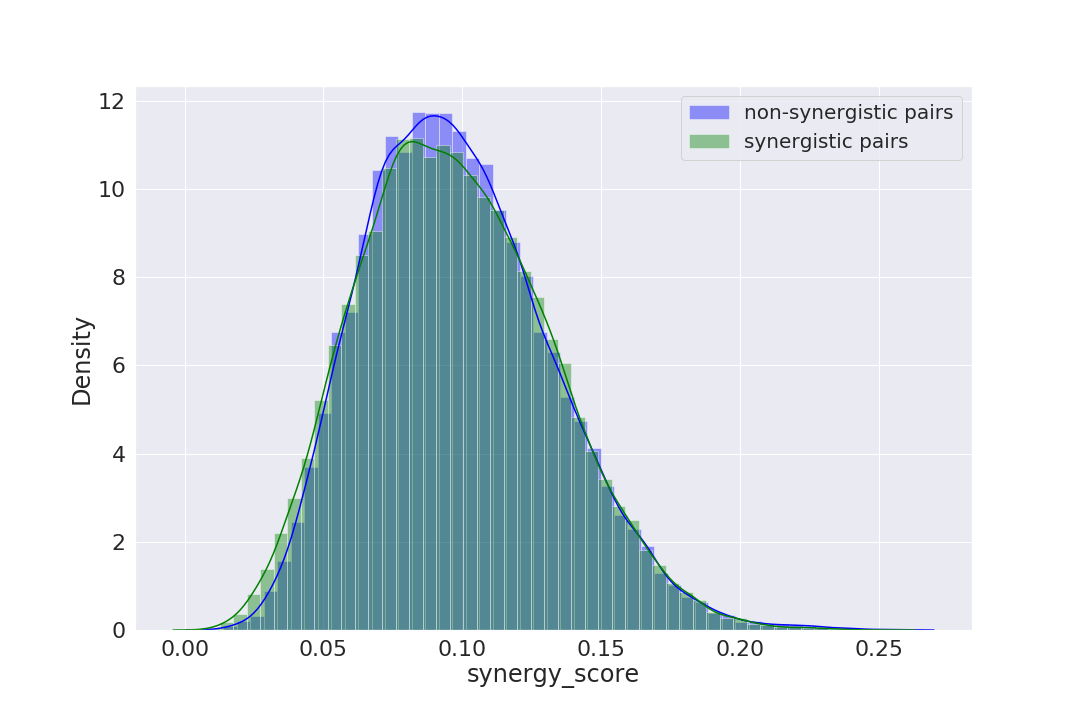
\includegraphics[width=1\linewidth]{images/fig_tanimoto_coeff_Fibroblasts_Induced_Neurons_opt_big_label.png}} \\b)
\end{minipage}
\vfill
\begin{minipage}[h]{0.5\linewidth}
\center{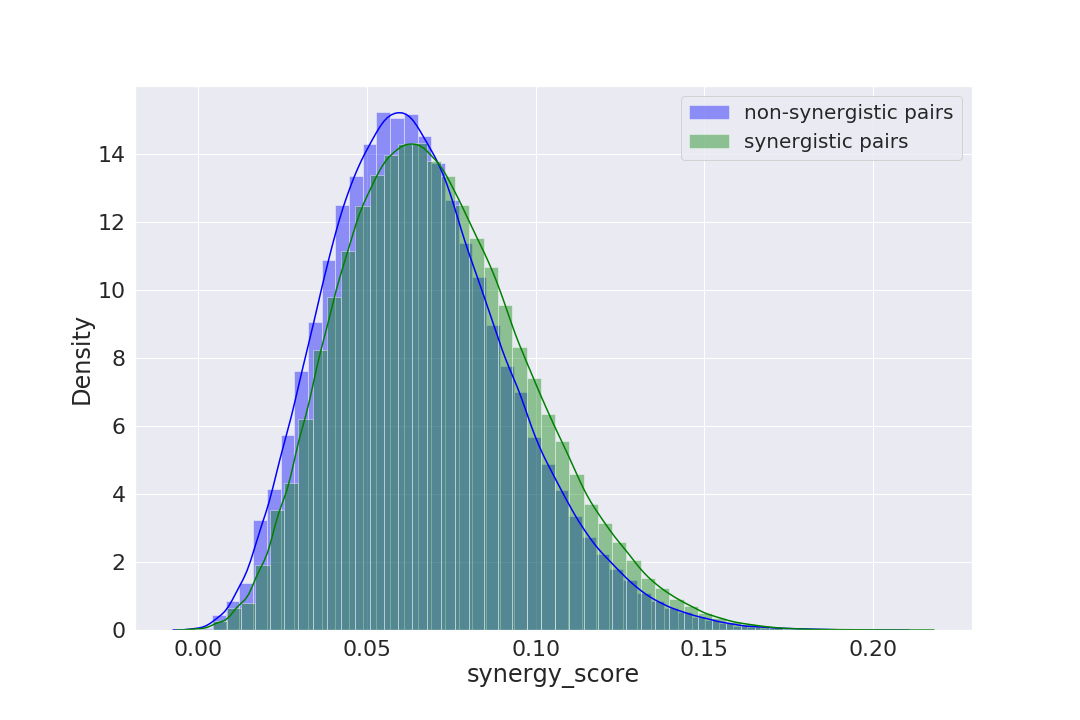
\includegraphics[width=1\linewidth]{images/fig_tanimoto_coeff_Fibroblasts_Induced_Neural_Stem_Cells_opt_big_label.png}} c) \\
\end{minipage}
\hfill
\begin{minipage}[h]{0.5\linewidth}
\center{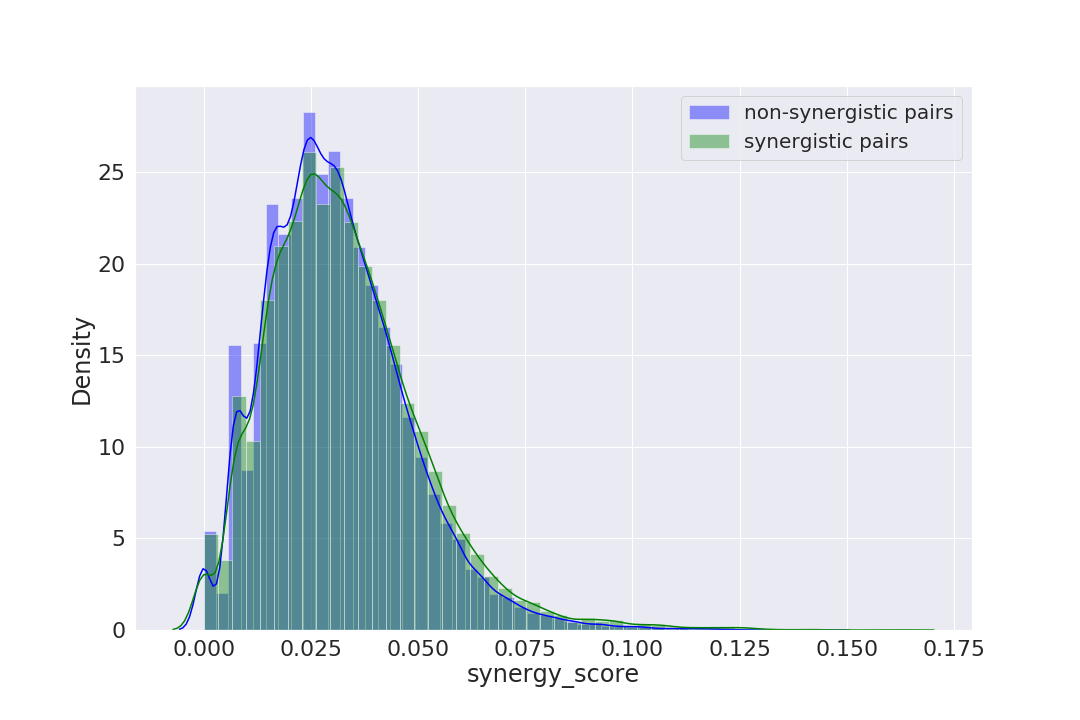
\includegraphics[width=1\linewidth]{images/fig_tanimoto_coeff_Fibroblasts_Induced_Pancreatic_Beta_Cells_opt_big_label.png}} d) \\
\end{minipage}
\vfill
\begin{minipage}[h]{0.5\linewidth}
\center{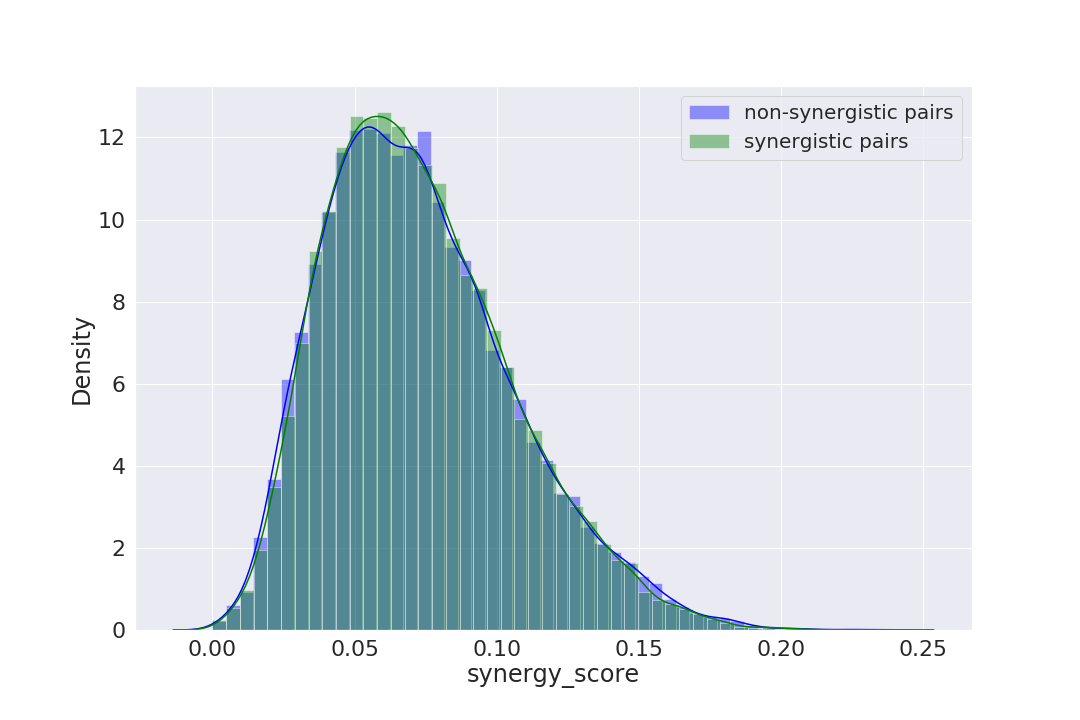
\includegraphics[width=1\linewidth]{images/fig_tanimoto_coeff_Mesenchymal_Stem_Cells_Induced_Neurons_opt_big_label.png}} e) \\
\end{minipage}
\hfill
\begin{minipage}[h]{0.5\linewidth}
\center{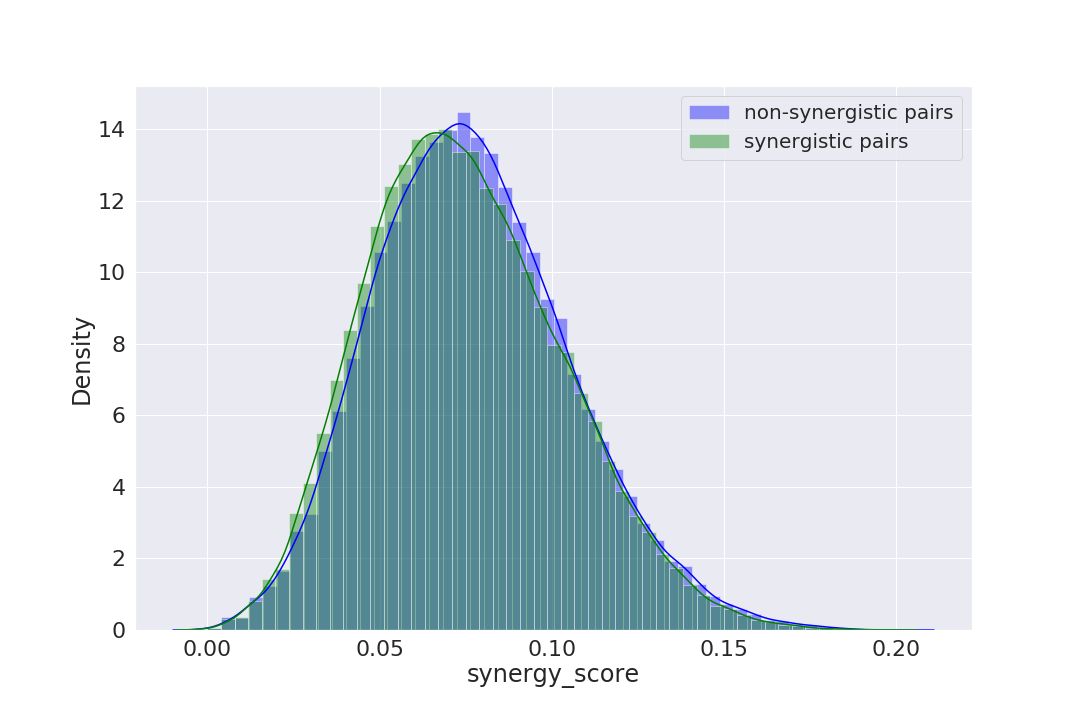
\includegraphics[width=1\linewidth]{images/fig_tanimoto_coeff_Fibroblasts_Induced_Pluripotent_Stem_Cells_opt_big_label.png}} f)
\end{minipage}
\caption{Распределение значений уровня синергии синергетических и несинергетических пар : a) фибробласты -> индуцированные кардиомиоциты, b)фибробласты -> индуцированные нейроны c) фибробласты -> индуцированные нейральные стволовые клетки, d)  фибробласты -> индуцированные $ \beta$-клетки поджелудочной железы, e) мезенхимальные стволовые клетки -> индуцированные нейроны, f) фибробласты -> индуцированные плюрипотентные стволовые клетки }
\label{tanimoto}
\end{figure}
\subsubsection{С использованием взаимной информации}
Данный подход основан на гипотезе, что синергетические малые молекулы активируют или подавляют одни и те же сигнальные пути (гипотеза сходства). Была проведена валидация метода и ее результаты приведены в таблице \ref{MI_table}.

\begin{table}[h]
    \caption{Результаты валидации}
    \centering
    \begin{tabular}{|c|c|c|c|c|c|c|c|}
    \hline
\makecell{№ кл. \\перех.}  &  \makecell{разн.\\ ср. знач.} &       p\_value &  \makecell{число\\ синерг.\\ пар \\в топ 50 }&  \makecell{число\\ пар} &  \makecell{число\\ синерг.\\ пар \\в топ 5\% }& \makecell{ число\\ пар \\в топ 5\% }&  \makecell{доля \\синерг.\\ пар\\ в топ 5\%} \\
    \hline
1 &           0.0573 &  0 &                          29 &    1236378 &                   33222 &           61819 &               0.537 \\
 \hline
2 &           0.0097 &  3.840e-21 &                          41 &      71631 &                    2565 &            3582 &               0.716\\
 \hline
3 &          -0.2091 &  0&                          24 &     475800 &                   15174 &           23790 &               0.638 \\
 \hline
4 &           0.0156 &  4.804e-06 &                          22 &      74691 &                    1200 &            3735 &               0.321\\
 \hline
5 &           0.0023 &  1.7023e-11 &                          40 &      49770 &                    1708 &            2488 &               0.686 \\
 \hline
6 &          -0.0257 &  1.202e-18 &                          36 &     128778 &                    4067 &            6439 &               0.632 \\
\hline
    \end{tabular}
    \label{MI_table}
\end{table}

Для этого метода есть 2 отрицательных значения для разницы средних значений уровня синергии синергетических и несинергетических выборок. То есть данных подход показал лучше результаты, по сравнению с тем, который основан на гипотезе комплементарности. 


На рисунке \ref{mutual_info} показаны распределения значений уровня синергии для синергетических пар и несинергетических пар.
\begin{figure}[H]
\begin{minipage}[h]{0.5\linewidth}
\center{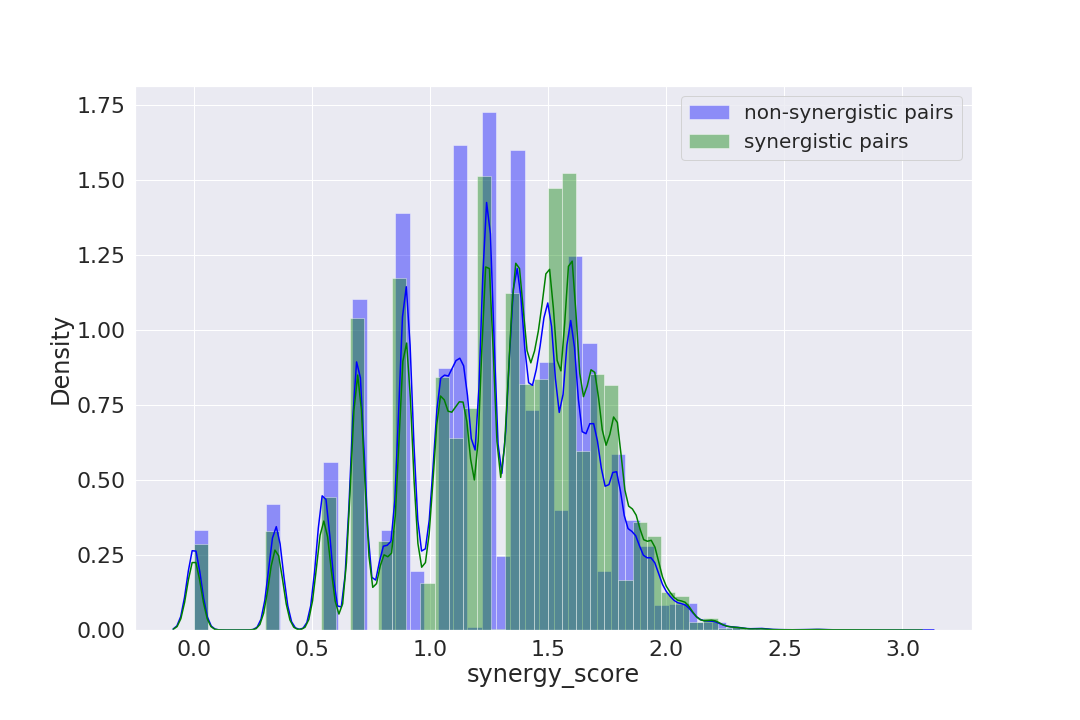
\includegraphics[width=1\linewidth]{images/fig_mutual_info_coeff_Fibroblasts_Induced_Cardiomyocytes_opt_big_label.png}} a) \\
\end{minipage}
\hfill
\begin{minipage}[h]{0.5\linewidth}
\center{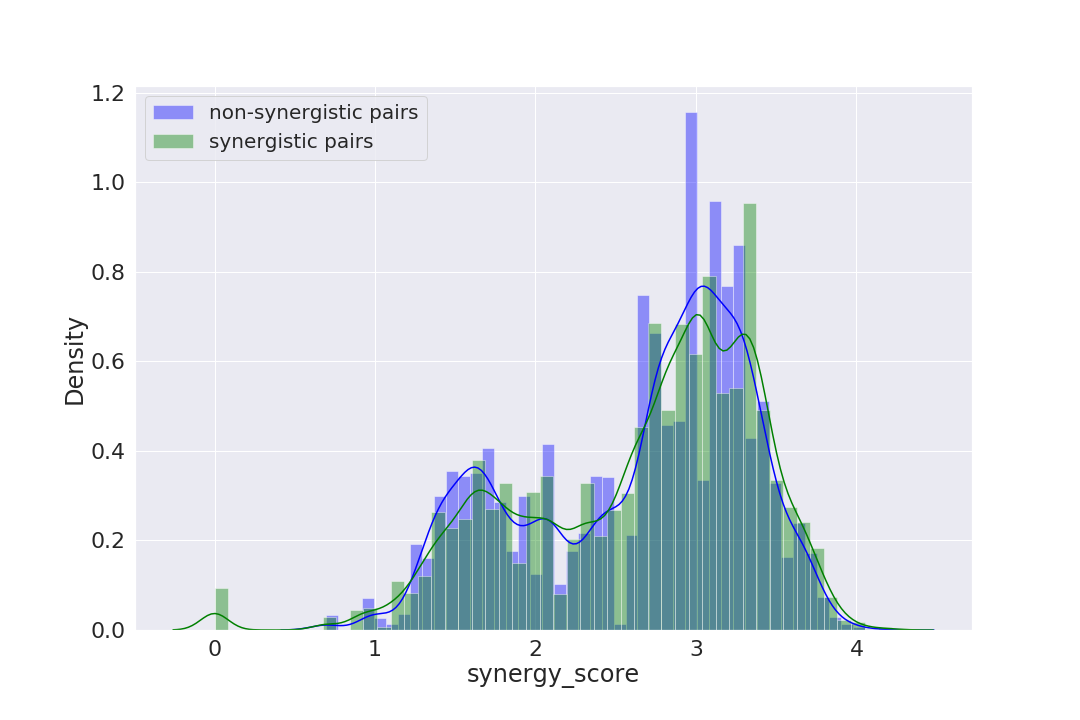
\includegraphics[width=1\linewidth]{images/fig_mutual_info_coeff_Fibroblasts_Induced_Neurons_opt_big_label.png}} \\b)
\end{minipage}
\vfill
\begin{minipage}[h]{0.5\linewidth}
\center{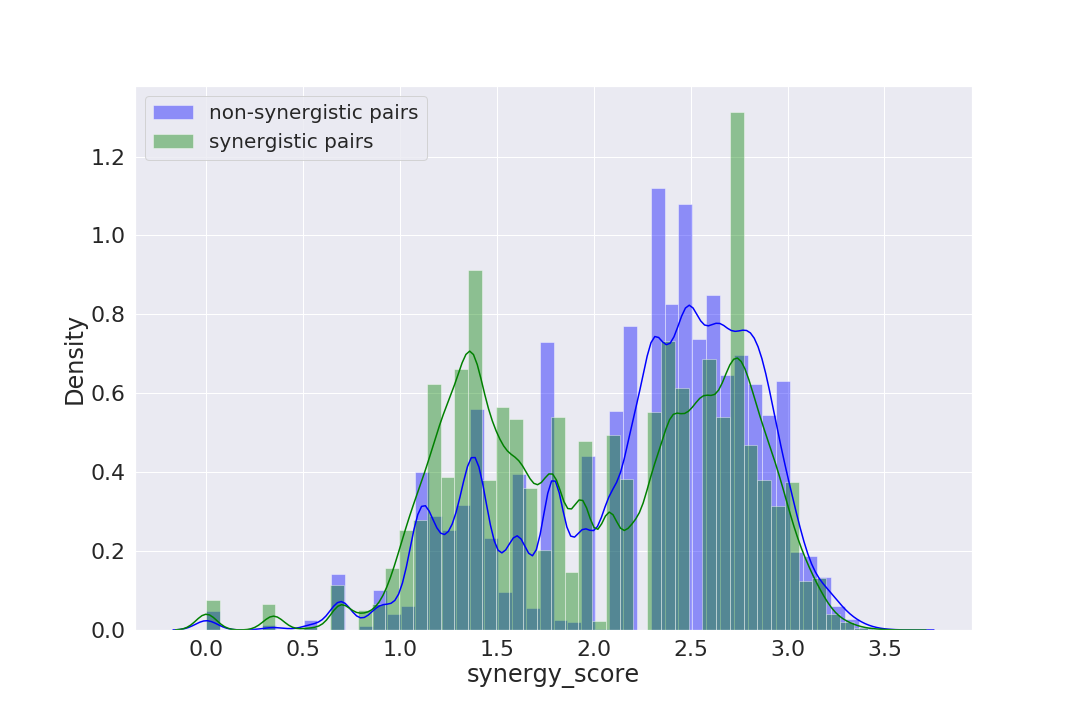
\includegraphics[width=1\linewidth]{images/fig_mutual_info_coeff_Fibroblasts_Induced_Neural_Stem_Cells_opt_big_label.png}} c) \\
\end{minipage}
\hfill
\begin{minipage}[h]{0.5\linewidth}
\center{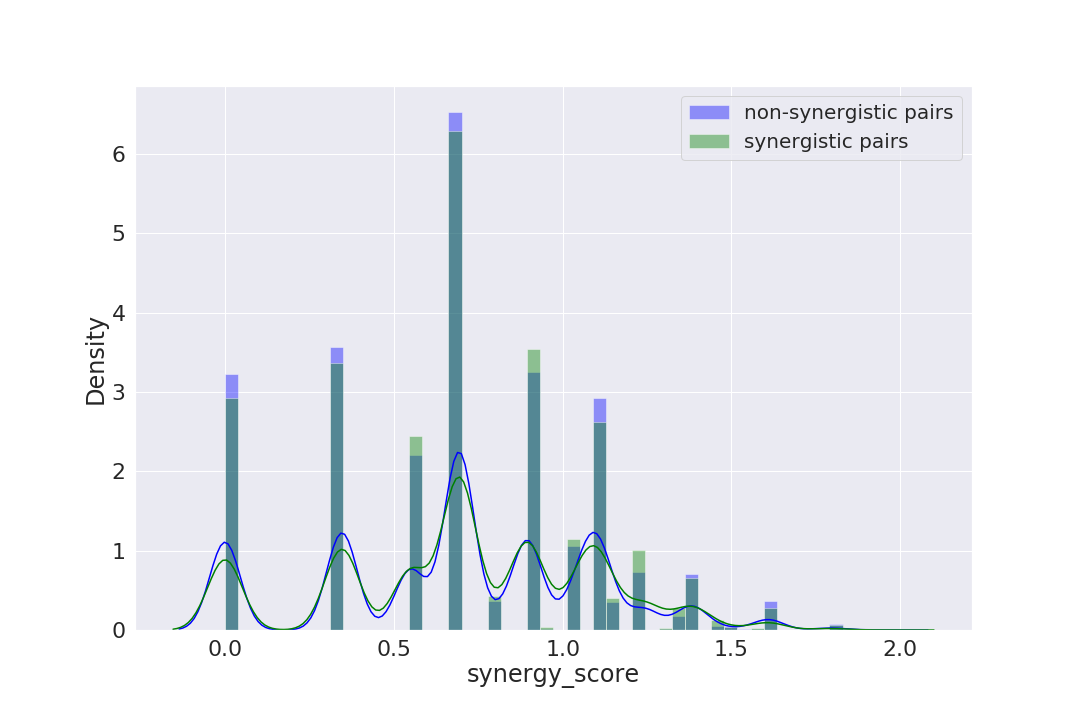
\includegraphics[width=1\linewidth]{images/fig_mutual_info_coeff_Fibroblasts_Induced_Pancreatic_Beta_Cells_opt_big_label.png}} d) \\
\end{minipage}
\vfill
\begin{minipage}[h]{0.5\linewidth}
\center{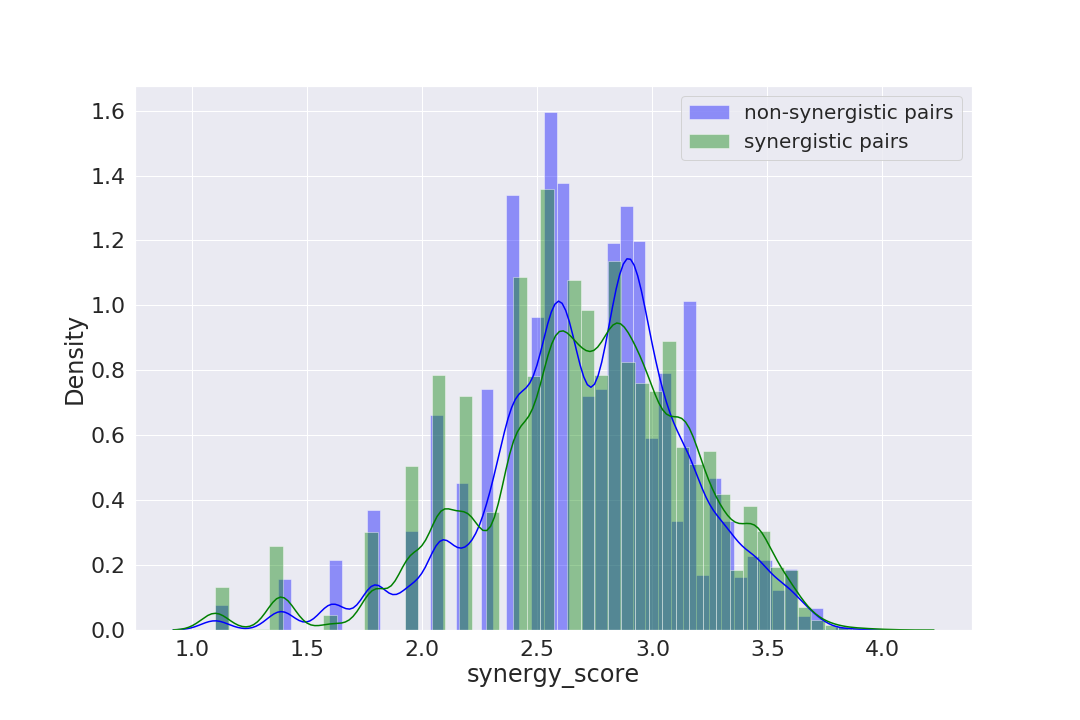
\includegraphics[width=1\linewidth]{images/fig_mutual_info_coeff_Mesenchymal_Stem_Cells_Induced_Neurons_opt_big_label.png}} e) \\
\end{minipage}
\hfill
\begin{minipage}[h]{0.5\linewidth}
\center{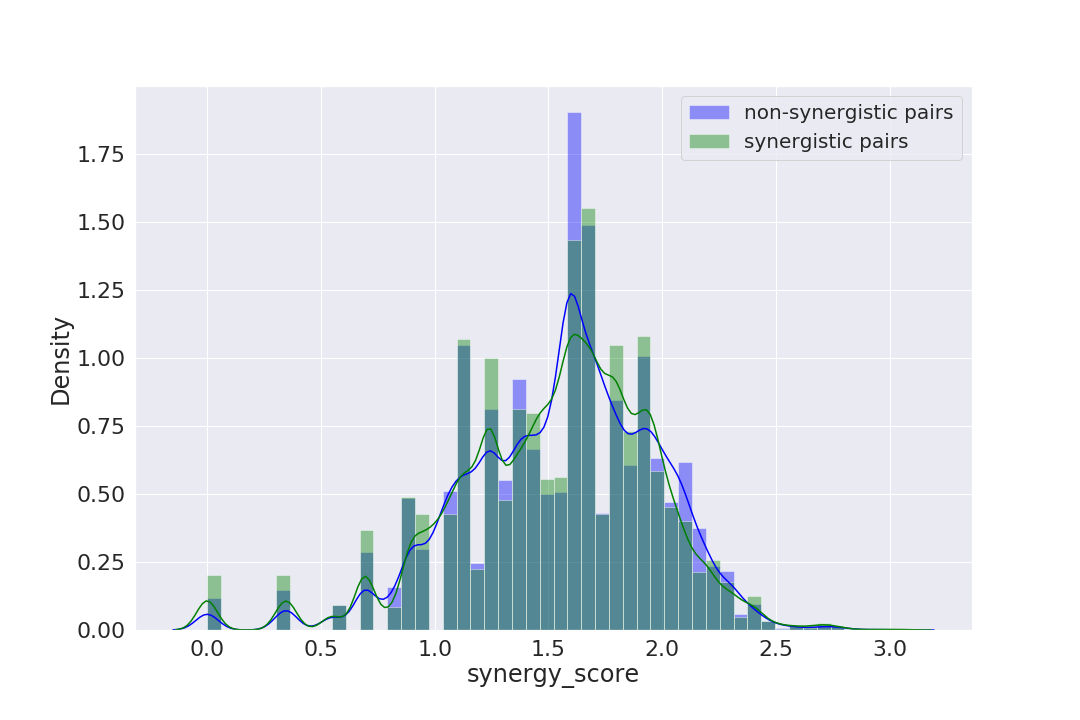
\includegraphics[width=1\linewidth]{images/fig_mutual_info_coeff_Fibroblasts_Induced_Pluripotent_Stem_Cells_opt_big_label.png}} f)
\end{minipage}
\caption{Распределение значений уровня синергии синергетических и несинергетических пар : a) фибробласты -> индуцированные кардиомиоциты, b)фибробласты -> индуцированные нейроны c) фибробласты -> индуцированные нейральные стволовые клетки, d)  фибробласты -> индуцированные $ \beta$-клетки поджелудочной железы, e) мезенхимальные стволовые клетки -> индуцированные нейроны, f) фибробласты -> индуцированные плюрипотентные стволовые клетки }
\label{mutual_info}
\end{figure}